\documentclass[10pt,landscape,a4paper]{article}
\usepackage[utf8]{inputenc}
\usepackage[ngerman]{babel}
\usepackage{tikz}
\usepackage{setspace}
\usetikzlibrary{shapes,positioning,arrows,fit,calc,graphs,graphs.standard}
\usepackage[nosf]{kpfonts}
\usepackage[t1]{sourcesanspro}
%\usepackage[lf]{MyriadPro}
%\usepackage[lf,minionint]{MinionPro}
\usepackage{multicol}
\usepackage{wrapfig}
\usepackage[top=2mm,bottom=2mm,left=2mm,right=2mm]{geometry}
\usepackage[framemethod=tikz]{mdframed}
\usepackage{microtype}
\usepackage{amsmath}
\usepackage{tcolorbox}
\usepackage{pdfpages}

\let\bar\overline

\definecolor{myblue}{cmyk}{1,.72,0,.38}

\def\firstcircle{(0,0) circle (1.5cm)}
\def\secondcircle{(0:2cm) circle (1.5cm)}

\colorlet{circle edge}{myblue}
\colorlet{circle area}{myblue!5}

\tikzset{filled/.style={fill=circle area, draw=circle edge, thick},
    outline/.style={draw=circle edge, thick}}

\pgfdeclarelayer{background}
\pgfsetlayers{background,main}

\everymath\expandafter{\the\everymath \color{myblue}}
\everydisplay\expandafter{\the\everydisplay \color{myblue}}

\renewcommand{\baselinestretch}{.8}
\pagestyle{empty}

\global\mdfdefinestyle{header}{%
linecolor=gray,linewidth=1pt,%
leftmargin=0mm,rightmargin=0mm,skipbelow=0mm,skipabove=0mm,
}

\newcommand{\header}{
\begin{mdframed}[style=header]
\footnotesize
\sffamily
Falls nicht anders angegeben: $A \in \mathbf{R}^{nxm}$ und $x,y \in \mathbf{R}$, ex. = existiert \hspace*{8mm} Seite ~\thepage~
\end{mdframed}
}

\makeatletter
\renewcommand{\section}{\@startsection{section}{1}{0mm}%
                                {.2ex}%
                                {.2ex}%x
                                {\color{myblue}\sffamily\small\bfseries}}
\renewcommand{\subsection}{\@startsection{subsection}{1}{0mm}%
                                {.2ex}%
                                {.2ex}%x
                                {\sffamily\bfseries}}



\def\multi@column@out{%
   \ifnum\outputpenalty <-\@M
   \speci@ls \else
   \ifvoid\colbreak@box\else
     \mult@info\@ne{Re-adding forced
               break(s) for splitting}%
     \setbox\@cclv\vbox{%
        \unvbox\colbreak@box
        \penalty-\@Mv\unvbox\@cclv}%
   \fi
   \splittopskip\topskip
   \splitmaxdepth\maxdepth
   \dimen@\@colroom
   \divide\skip\footins\col@number
   \ifvoid\footins \else
      \leave@mult@footins
   \fi
   \let\ifshr@kingsaved\ifshr@king
   \ifvbox \@kludgeins
     \advance \dimen@ -\ht\@kludgeins
     \ifdim \wd\@kludgeins>\z@
        \shr@nkingtrue
     \fi
   \fi
   \process@cols\mult@gfirstbox{%
%%%%% START CHANGE
\ifnum\count@=\numexpr\mult@rightbox+2\relax
          \setbox\count@\vsplit\@cclv to \dimexpr \dimen@-1cm\relax
\setbox\count@\vbox to \dimen@{\vbox to 1cm{\header}\unvbox\count@\vss}%
\else
      \setbox\count@\vsplit\@cclv to \dimen@
\fi
%%%%% END CHANGE
            \set@keptmarks
            \setbox\count@
                 \vbox to\dimen@
                  {\unvbox\count@
                   \remove@discardable@items
                   \ifshr@nking\vfill\fi}%
           }%
   \setbox\mult@rightbox
       \vsplit\@cclv to\dimen@
   \set@keptmarks
   \setbox\mult@rightbox\vbox to\dimen@
          {\unvbox\mult@rightbox
           \remove@discardable@items
           \ifshr@nking\vfill\fi}%
   \let\ifshr@king\ifshr@kingsaved
   \ifvoid\@cclv \else
       \unvbox\@cclv
       \ifnum\outputpenalty=\@M
       \else
          \penalty\outputpenalty
       \fi
       \ifvoid\footins\else
         \PackageWarning{multicol}%
          {I moved some lines to
           the next page.\MessageBreak
           Footnotes on page
           \thepage\space might be wrong}%
       \fi
       \ifnum \c@tracingmulticols>\thr@@
                    \hrule\allowbreak \fi
   \fi
   \ifx\@empty\kept@firstmark
      \let\firstmark\kept@topmark
      \let\botmark\kept@topmark
   \else
      \let\firstmark\kept@firstmark
      \let\botmark\kept@botmark
   \fi
   \let\topmark\kept@topmark
   \mult@info\tw@
        {Use kept top mark:\MessageBreak
          \meaning\kept@topmark
         \MessageBreak
         Use kept first mark:\MessageBreak
          \meaning\kept@firstmark
        \MessageBreak
         Use kept bot mark:\MessageBreak
          \meaning\kept@botmark
        \MessageBreak
         Produce first mark:\MessageBreak
          \meaning\firstmark
        \MessageBreak
        Produce bot mark:\MessageBreak
          \meaning\botmark
         \@gobbletwo}%
   \setbox\@cclv\vbox{\unvbox\partial@page
                      \page@sofar}%
   \@makecol\@outputpage
     \global\let\kept@topmark\botmark
     \global\let\kept@firstmark\@empty
     \global\let\kept@botmark\@empty
     \mult@info\tw@
        {(Re)Init top mark:\MessageBreak
         \meaning\kept@topmark
         \@gobbletwo}%
   \global\@colroom\@colht
   \global \@mparbottom \z@
   \process@deferreds
   \@whilesw\if@fcolmade\fi{\@outputpage
      \global\@colroom\@colht
      \process@deferreds}%
   \mult@info\@ne
     {Colroom:\MessageBreak
      \the\@colht\space
              after float space removed
              = \the\@colroom \@gobble}%
    \set@mult@vsize \global
  \fi}

\newcommand{\mybox}{%
    \collectbox{%
        \setlength{\fboxsep}{1pt}%
        \fbox{\BOXCONTENT}%
    }%
}

\makeatother
\setlength{\parindent}{0pt}
\renewcommand*\arraystretch{1.0}
\renewcommand*{\arraycolsep}{0.5mm}

\begin{document}
\small
\begin{multicols*}{5}
\section{Matrix Eigenschaften}
\textbf{invertierbar} $\Leftrightarrow$ \textbf{regulär}: $AB = BA = I_{N}$\\
\textbf{symmetrisch}.: $(AB)^{T} = B^{T}*A^{T} = BA$\\
\textbf{EW $\lambda$}: $Av = \lambda v$\\ 
$\sigma(A)$: \textbf{Spektrum}, alle EW\\
\textbf{orthogonal}: $A^T = A^{-1} \Rightarrow A^T * A = I_N$,\\
längenerhaltend $||Qx||_2^2 = ||x||_2^2$\\
\textbf{ähnlich}: $A = SBS^{-1}$
\subsection*{Skalarprodukt}
$||\cdot||$ heißt Norm falls: \\
1) $||x|| \geq 0$ (pos. definit)\\
2) $||x + y|| \leq ||x|| + ||y||$ (Dreiecksungl.)\\
3) $||\lambda x|| = |\lambda| ||x||$ (Homogenität)\\

$\langle \cdot , \cdot \rangle$ heißt Skalarprodukt, falls:\\
$\langle \lambda x + \mu y , z \rangle = \lambda\langle x , z \rangle + \mu\langle y , z \rangle$\\
$\langle x , y \rangle = \langle y , x \rangle$\\
$\langle x , x \rangle \geq 0 $ und $\langle x , x \rangle = 0 \Leftrightarrow x = 0$\\
Es gilt: 1) $||x|| := \sqrt{\langle x , x \rangle}$\\
2) $|\langle x , y \rangle| \leq ||x|| ||y||$\\
3) $\langle x , y \rangle_{A} = x^{T}Ay$, A: spd-Matrix

\input{content/Einführung}
\section{Lösungsverfahren}
Finde x, sodass $Ax = b$, wobei $A \in \mathbb{R}^{NxN}$\\
$x = A^{-1}b \rightarrow$ teuer\\
Falls Matrix nicht regulär $\rightarrow$ keine oder inf. Lösungen. A regulär $\leftrightarrow$ det(A) $\neq$ 0\\
Es gilt: det(A) = det(L) * det(R)
\subsection{LR-Zerlegung}
1) \textbf{Zerlegung}: $A = LR$ ($\approx \frac{N^3}{3}$)\\
2) \mbox{\textbf{Vorwärtssubstitution}: $Ly = b$} ($\approx \frac{N^2}{2}$)\\
3) \mbox{\textbf{Rückwärtssubstitution}: $Rx = y$ ($\approx \frac{N^2}{2}$)}\\
\textbf{Begründung}: $Ax = LRx = Ly = b$\\
Eine LR-Zerlegung existiert $\leftrightarrow$ Jede Teilmatrix ($A_{[1:n,1:n]}$) ist regulär (eindeutig)\\
\textbf{Vorgehensweise}: Matrix gaußen, Gaußschritte mit \textbf{umgekehrtem} Vorzeichen an der jeweiligen Stelle speichern.\\
\textbf{L}: Diagonale = 1, untere DEM = Gauß\\
\textbf{R}: untere DEM = 0, Rest = Gauß-Matrix\\
\mbox{\textbf{Permutation}: $A$ regulär $\leftrightarrow PA = LR$}\\
\mbox{$PA = LR \Rightarrow A^TP^T = R^TL^T$, $b = R^TL^T(Px)$}\\
$A = LR$ existiert nicht immer, $PA = LR$ schon falls \textbf{A invertierbar} ist.\\
$Ax = b \Leftrightarrow PAx = Pb \Leftrightarrow LRx = Ly = Pb$\\
\textbf{Spaltenpivotwahl} immer machen, Betragsmäßig größtes Element kommt nach oben, bei Gleichheit egal

\subsection{Cholesky-Zerlegung}
A ist spd-Matrix $\Leftrightarrow$ Cholesky Z. existiert\\
\textbf{Aufwand}: $\sum_{n=1}^{N-1}\frac{n^2}{2} \approx \frac{N^3}{6}$ Operationen\\
1) \textbf{Zerlegung}: $A = LL^T$\\
2) \textbf{VWS}: $Ly = b$, 
3) \textbf{RWS}: $L^Tx = y$\\
$A^T = (LL^T)^T = (L^T)^TL^T = LL^T = A$\\
\mbox{$x^TAx = x^TLL^Tx = (L^Tx)^TL^Tx = y^Ty > 0$}\\
Für eine 4x4-Matrix gilt:\\
$l_{11} = \sqrt{a_{11}}$ \textbf{;} $l_{21} = \frac{a_{21}}{l_{11}}$, $l_{22} = \sqrt{a_{22} - l^2_{21}}$ \textbf{;}\\
$l_{31} = \frac{a_{31}}{l_{11}}$, $l_{32} = \frac{a_{32}-l_{31}l_{21}}{l_{22}}$,\\ $l_{33} = \sqrt{a_{33} - (l^2_{31} + l^2_{32})}$ \textbf{;}\\
$l_{41} = \frac{a_{41}}{l_{11}}$,
$l_{42} = \frac{a_{42}-l_{41}l_{21}}{l_{22}}$,\\
$l_{43} = \frac{a_{43}-l_{41}l_{31} + l_{42}l_{32}}{l_{33}}$,\\ $l_{44} = \sqrt{a_{44} - (l^2_{41} + l^2_{42} + l^2_{43})}$\\
\textbf{Tipp}: Bandstruktur bleibt erhalten
\subsection{QR-Zerlegung} 
Sei A eine MxN Matrix $\Leftrightarrow A = QR$, wobei $Q \in \mathbb{R}^{MxM}$ orthogonal ($QQ^T = I_M$) und  $R \in \mathbb{R}^{NxN}$ eine obere Dreiecksmatrix.\\
1) \textbf{Householder-Trans}: $A = QR$\\
2) \textbf{Löse}: $Qc = b$ durch $c = Q^Tb$\\
3) \textbf{Rückwärtssubstitution}: $Rx = c$\\
\textbf{Begründung}: $Ax = QRx = Qc = b$\\
\mbox{\textbf{Eigenschaften}: stabil, $\frac{2}{3}N^3$ wenn $M \approx N$}\\
$Q = I_M - 2ww^T$ wobei $w \in \mathbb{R}^M$, $w^Tw = 1$\\
Q ist sym. da $Q^T = I_M^T - (2ww^T)^T = Q$,
orthogonal da $QQ^T = Q^2 = I_M -4ww^T + 4w * 1 * w^T = I_M (w^Tw = 1)$, Spiegelung da $Q\lambda w = -\lambda w$ für $w^Ty = 0 \rightarrow Qy = y$\\
\textbf{Ziel}: $H^{(k)}*...*H^{(1)}*A = R$, wobei $H^{(n)}$ orthogonal\\
\textbf{Schritte}: $v^{(1)} = q_1 + sgn(a_{11}) * ||a_1|| * e_1$\\
$H^{(1)} = H^{(0)} = I - \frac{2v^{(1)}v^{(1)^T}}{v^{(1)^T}v^{(1)}}$\\
$A^{(1)} = H^{(1)}*A$\\
Erste Zeile und Spalte streichen\\
$H^{(2)}$ in der ersten Zeile und Spalte um $e_1$ erweitern\\
$H^{(2)} = H^{(2)}A^{(1)}$ ... Für R: (m-1) mal\\
$Q^T = H^{(2)}H^{(1)} \rightarrow Q = (Q^T)^T$ 

\subsection{Kondition}
Empfindlichkeit von Matrix-Störungen\\
Sei $A \in \mathbb{R}^{NxN}$ nachfolgend regulär:\\
\textbf{zugehörige Norm}: $||A|| := sup\frac{||Ax||}{||x||}$, $x \neq 0$\\
Es gilt: $||I_N|| = 1$ und $||AB|| \leq ||A|| * ||B||$\\
\mbox{\textbf{SSN}: $||A||_1 = \underset{m = 1,...,N}{max}\sum_{n=1}^N|a_{nm}|$}\\
\mbox{\textbf{Spektral}: $||A||_2 = \sqrt{\text{größter EW von } A^TA}$}\\
\mbox{\textbf{ZSN}: $||A||_{\infty} = \underset{n=1,...,N}{max}\sum_{m=1}^N|a_{nm}|$}\\
${||x - \widetilde{x}}|| = ||A^{-1}(b - \widetilde{b})|| \leq ||A^{-1}|| * ||b-\widetilde{b}||$: (absoluter Fehler), (relativer Fehler):\\
$\frac{||x - \widetilde{x}||}{||x||} \leq ||A||*||A^{-1}||*\frac{||b-\widetilde{b}||}{||b||}$\\
\textbf{Konditionszahl}: $cond(A) := ||A||*||A^{-1}||$\\
\textbf{Eigenschaften}: $1 \leq cond(A)$, $cond(A) = \\cond(\alpha A)$, mit \mbox{$\alpha \neq 0$, $cond(A) = cond(A^{-1})$}\\
$cond(A) = \frac{max_{||y|| = 1}||Ay||}{min_{||z|| = 1}||Az||}$ (allg. Definition)\\
Matrizen $B^TB$ wobei B beliebig:\\
- sind spezielle sym. Matrizen\\
- haben nur nichtnegative (inkl. 0) EW\\
- nur positive EW falls B maximaler Rang\\
- besitzen EW $\lambda^2$ falls B sym. mit EW $\lambda$\\
$\Rightarrow cond_2(A) = \frac{max\{|\lambda|:\; \lambda \text{ EW von A}\}}{min\{|\lambda|:\; \lambda \text{ EW von A}\}}$\\
\mbox{Sei $\frac{||A-\widetilde{A}||}{||A||} \leq \epsilon_A$ und $\frac{||b-\widetilde{b}||}{||b||} \leq \epsilon_b$, dann gilt:}\\
\mbox{$\frac{||x-\widetilde{x}||}{||x||} \leq \frac{cond(A) * (\epsilon_A + \epsilon_b)}{1-\epsilon_A * cond(A)}$, $\epsilon_A * cond(A) < 1$}\\ 
\textbf{gute Kondition}: $I_n$ ($cond(A)_2$ = 1),\\ $||\text{orthogonale Matrizen}||_2 = 1$, Spline-\\ \mbox{Interpol., $cond(A)$ klein $\Rightarrow$ LGS gut kond.}\\
\textbf{schlechte Kondition}: Hilbertmatrix, \mbox{Diagonalmatrix* ($cond_2(A) = \frac{max.\; EW}{min.\; EW}$)}

\mbox{\textbf{Neumann-Reihe}: $(I_n + B)^{-1} = \sum_{k=0}^\infty (-B)^k$}

\subsection{Ausgleichsrechnung}
$x$ gesucht, sodass $||Ax-b||_2 = min!$ mit $A \in \mathbb{R}^{MxN}$
Falls $M=N$ gilt: $||Ax-b||_2 = 0 = min! \;(Ax = b)$\\
\textbf{Satz von Gauß}: Der Vektor x löst genau dann das lineare AGP, falls er \mbox{$A^TAx = A^Tb$ löst (Normalengleichung}\\
NG immer lösbar falls $Rang(A) = max$, da $A^Tb \in Bild(A^T) = Kern(A)^{\bot} = Kern(A^TA)^{\bot} = Bild(A^TA)$, in $N^2 + \frac{1}{2}N^2$\\
Sei $A \in \mathbb{R}^{MxN}$ mit $M \geq N$ und $Q, R$ die QR-Zerlegung, also $Q^TA = R = \begin{pmatrix} \overline{R} \\ 0 \end{pmatrix}$, dann ist $x = \overline{R}^{-1}c$ die Lsg. des AGPs, wobei $Q^Tb = \begin{pmatrix} c \\ d \end{pmatrix}$, \textbf{Householder: $A = QR$,
\textbf{Löse}: $Q^Tb = \begin{pmatrix} c \\ d \end{pmatrix}$}, \textbf{RWS}: $\overline{R}x = c$
\subsection{Singulärwertzerlegung}
Sei $A \in \mathbb{R}^{MxN}$ mit Rang $r$,
\textbf{Zerlegung}: $A = U * \Sigma * V^T$, wobei $U \in \mathbb{R}^{MxM}$ und $V \in \mathbb{R}^{NxN}$ orthogonal,  $\Sigma \in \mathbb{R}^{MxN}$ mit Singulärwerten ($s_n \geq ... \geq s_r > 0$)\\
\begin{onehalfspace}$AA^T = U\Sigma V^TV\Sigma^TU^T = U\Sigma \Sigma^TU^T$ und\\
$A^TA = V\Sigma^TU^TU\Sigma V^T = V\Sigma^T \Sigma V^T$
\end{onehalfspace}
\textbf{Beispiel $U' = A*A^T$, $V' = A^T*A$}:
\[ A = \left( \begin{array}{cc}
1 & 0 \\
0 & 1 \\
1 & 1
\end{array} \right)
\rightarrow \Sigma =
\left( \begin{array}{cc}
s_1 & 0 \\
0 & s_2 \\
0 & 0
\end{array} \right) , U' = 
\left(\begin{array}{ccc}
1 & 0 & 1\\
0 & 1 & 1\\
1 & 1 & 2
\end{array} \right)\]
\mbox{$\lambda_1 = 3 (s_1 = \sqrt{3})$, $\lambda_2 = 1 (s_2 = \sqrt{1})$, $\lambda_3 = 0$}\\
Eigenräume ausrechnen, analog mit \\$V'$. V und U sind normierte Eigenräume.\\
$||A||_{Frob} = \sqrt{Spur(A^TA)} = \sqrt{\sigma_1^2 + ... + \sigma_r^2}$
\section{Newton-Verfahren}
Lösungsverfahren für nichtlineare GS\\
\textbf{Gesucht x*}: $f(x^*) = 0_N$, f nichtlinear,
$f_1(x_1^*, ..., x_N^* = 0)$, ..., $f_N(x_1^*, ..., x_N^* = 0)$\\
\mbox{\textbf{Taylor}: $0 = f(x^*) = f(x^0) + f'(x^0)(x^* - x^0)$}\\
\textbf{Algorithmus}:\\
1) Wähle Startwert $x^0$ und Toleranz $\epsilon$\\
2) Löse $f'(x^k)d^k = -f(x^k)$ (LGS,\\ LR-Zerlegung), berechne $x^{k+1} = x^k + d^k$
3) Falls ($||d^k|| < \epsilon$): STOP, ansonsten 2)\\
\textbf{Bemerkung}: Konv. \textbf{lokal} quadratisch\\
Oft divergent, falls $||x^0 - x^*||$ groß\\
\textbf{Konvergenz}: $||x^* - x^k|| \leq C||x^*-x^{k-1}||^2$, d.h. die Anzahl an Nachkommastellen verdoppelt sich ca. pro Schritt\\
\textbf{Funktionen}: $x_{n+1} = x_n - f'(x_n)^{-1}f(x_n)$
\subsection{Vereinfachung}
Konstante Matrix A, sodass $A \approx f'(x^0)$, dann gilt $F(x) = x - A^{-1}f(x)$.\\
1 x LR-Zerlegung, \textbf{linear konvergent}\\
\textbf{Fixpunkt}: $x^{k+1} = x^k-A^{-1}f(x^k) = F(x^k)$


\section{Interpolation}
Stützpunkte $f_n$ gegeben, Funktion $p$\\ gesucht für die $p(x_n) = f_n$ und\\
$\int_a^b (f(x) - p(x))^2dx = min!$ gilt\\
\subsection{Polynom}
$N + 1$ Stützwerte, Poly. mit Grad $\leq N$ \\gesucht,
mit Grad $\leq N$ \textbf{eindeutig}\\
\textbf{Lagrange}: 
$L_n(x) = \underset{j = 0, j \neq n}{\prod^N}\frac{x-x_j}{x_n - x_j} $, instabil\\
$p(x) = \sum_{n=0}^N f_nL_n(x) \rightarrow$ sehr aufwändig
\textbf{Kondition}: Lebesgue-Konstante $\Lambda$\\
$\Lambda_N := \underset{x \in [a,b]}{max}\sum_{n=0}^N |L_n(x)|$,
großes $\Lambda_N$ bei hohem Grad und schlechten Stützstellen\\
\textbf{Newton-Darstellung}: $f_{n,n} = f_n$\\
$f_{n,k} = \frac{f_{n,k - 1} - f_{n + 1,k}}{x_n - x_k}$, $0 \leq n < k \leq N$\\

\textbf{Beispiel}:
\begin{tabular}{ c|c|c|c|c } 
 $f_n$ & 1 & 6 & -3 & 3\\ 
 \hline
 $x_n$ & -1 & 0 & 1 & 3\\ 
\end{tabular}
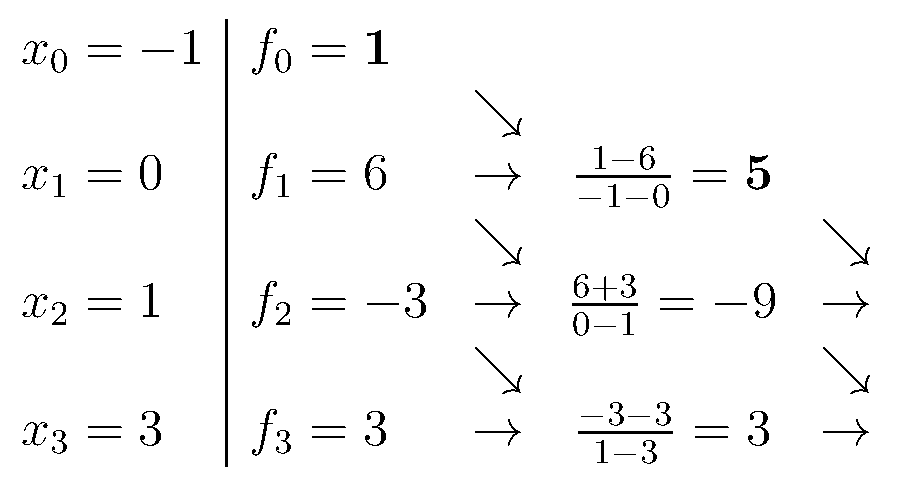
\includegraphics[scale=0.35]{content/images/Newton_Example.pdf}\\
$p = 1 + 5(x + 1)- 7(x + 1)x + \frac{11}{4}(x+1)x(x-1)$\\
\textbf{Aufwand}: $\frac{N(N + 1)}{2}$ Div, $N(N + 1)$ Add
\textbf{Fehler}: $f(x) - p(x) = w_{N+1}(x)*\frac{f^{(N+1)}(\xi)}{(N+1)!}$\\
$\rightarrow$ falls x Stützpunkt, dann 0\\
\textbf{Tschebyscheff}: Approximation von $f$ mit möglichst günstigen Stützstellen\\
$T_n(x) = cos(n*arccos(x))$ | $T_0(x) = 1$, $T_1(x) = x, T_{n+1}(x) = 2x * T_n(x) - T_{n-1}(x)$\\
$max_{x \in [-1, 1]}|w_{N+1}(x)$ min. mit $2^{-N}$\\
\textbf{Interpolationsformel}: $N + 1$ Stützstellen, eindeutiges Polynom gegeben durch:\\
$p(x) = \frac{1}{2}c_0 + c_1T_1(x) + ... + c_NT_N(x)$ mit
$c_m = \frac{2}{N + 1}\sum_{n=0}^N f_n cos(m * \pi * \frac{2n + 1}{2N + 2})$ für $m = 0,...,N$ ($(N + 1)^2$ Multiplikationen)\\
\textbf{Clenshaw-Algo}: Sei $d_{N+2} = d_{N+1} = 0$,\\
$d_n = c_n + 2x * d_{n+1} - d_{n+2}$ für $n = N, ...,0$
\mbox{$\rightarrow p(x) = \frac{(d_0 - d_2)}{2}$ ($N + 2$ Mul + $2N$ Add)}
\subsection{Kubische Splines}
Geg: Fallunterscheidung, Ges: $\mathbf{C}^2$-Funkt. mit Teilpolynomen $\in \mathbf{P}_3$ und $s(x_n) = y_n$
(Stützst.). ($s_n$ Teilpol., $x*$ Grenze) Ziel: \\
1) Glattheit. $s_n^{(k)}(x*) = s_{n+1}^{(k)}(x*)$, $k = 1, 2$\\
2) Interpolationsbed. $s_n(x*) = s_{n+1}(x*)$\\
\mbox{\textbf{Min-Eigenschaften}: \underline{Eine} Eigens. davon:}
1) $s^{\prime}(a) = \widetilde{s}^{\prime}(a)$ und $s^{\prime}(b) = \widetilde{s}^{\prime}(b)$\\
2) $s^{\prime\prime}(a) = 0$ und $s^{\prime\prime}(b) = 0$\\
3) $s^{(k)}(a) = s^{(k)}(b)$ für $k = 0,1,2$ und \hspace*{4mm} $\widetilde{s}^{\prime}(a) = \widetilde{s}^{\prime}(b)$\\
Sei s ein Spline, s heißt: \textbf{eingespannt}, \\
\textbf{hermitesch}: $s^{\prime}(a) = v_0$ und  $s^{\prime}(b) = v_N$\\
\textbf{natürlich}: $s^{\prime\prime}(a) = s^{\prime\prime}(b) = 0$\\
\mbox{\textbf{periodisch}: $s^{\prime}(a) = s^{\prime}(b)$ und $s^{\prime\prime}(a) = s^{\prime\prime}(b)$}\\
%\textbf{Not-a-knot}: $s_1'''(x_1) = s_2'''(x_1)$
\textbf{Minimalität}: $\int_a^b |s''(x)|^2 dx$ minimal\\
\textbf{Kondition}: $l_n(x)$ Lagrange-Spline:
\\$s(x) - \widetilde{s}(x) = \sum_{n=0}^{N}(y_n - \widetilde{y}_n)l_n(x)$\\
$\rightarrow$ gute Kondition, max. $\Lambda_N \leq 2$\\
äquidistanten Unterteilungen: hier gute Kondition, Polynom-Interpol. schlechte Kondition (Oszillationen etc.)

\section{Integration}
\textbf{Rechteckregel}: $I(f) \approx (b-a)f(a)$\\
\textbf{Mittelpunkt}: $I(f) \approx (b-a)f(\frac{a+b}{2})$\\
\textbf{Trapezregel}: $I(f) \approx (b-a)(\frac{f(a) + f(b)}{2})$\\
\mbox{\textbf{Simpson}: $I(f) \approx \frac{b-a}{6}(f(a) + 4f(\frac{a+b}{2}) + f(b))$}\\
- $\int_a^bf(x)dx = \int_a^cf(x)dx + \int_c^bf(x)dx$\\
- linear: $I(\lambda f + \mu g) = \lambda I(f) + \mu I(g)$\\
\mbox{- monoton: $f \geq g \Rightarrow \int_a^bf(x)dx \geq \int_a^bg(x)dx$}\\
$\rightarrow |\int_a^bf(x)dx| \leq \int_a^b|f(x)|dx$ (Bsp. Sinus)
\textbf{Kondition}: L1-Norm: $||f||_1 = I(|f|)$
Es gilt: $\frac{|I(f) - I(\widetilde{f})|}{|(f)|} \leq \frac{||f-\widetilde{f||_1}}{||f||_1}$ mit $cond_1 := \frac{I(|f|)}{|I(f)|}$ (monoton und linear), schlecht konditioniert falls oszillierend
\subsection{Quadraturformeln}
$\int_a^bf(x)dx \approx (b-a)\sum_{k=1}^s b_kf(a + c_k(b-a))$, $b_k$ Gewichte und $c_k$ Knoten $\in [0,1]$\\
linear und monoton $\leftrightarrow b_k \geq 0$, eindeutig\\
\textbf{Ordnung}: Quad.-Formel hat Ordnung p $\leftrightarrow$ QF liefert exakte Lösung für alle Poly. mit Grad $\leq p - 1$, wobei p maximal oder \\
(1) $\frac{1}{q} = \sum_{k=1}^sb_kc_k^{q-1}$ für alle $q = 1, ..., p$ aber nicht für $q = p + 1$ | $\updownarrow$ p mind. s \\
\textbf{Es gilt}: (2) $\sum_{k=1}^s b_k = 1$ | $b_k = \int_0^1 L_k(x)dx$\\
\textbf{Klausuren}: (1) und (2) überprüfen\\
\textbf{Kondition}: schlecht, da $\sum|b_k|$, k > 8
\subsection{sym. Quadraturformeln}
\mbox{QF sym. $\leftrightarrow c_k = 1 - c_{s+1-k}$ \& $b_k = b_{s+1-k}$}\\
Ordnung einer sym. QF ist \textbf{gerade}\\
\mbox{\textbf{Lagrange}: $L_{s+1-k}(x) = \underset{j=1, j \neq k}{\prod^s} \frac{x - c_{s+1 - j}}{c_{s+1-k} - c_{s+1-j}}$}

\subsection{QF mit erhöhter Ordnung}
Ges: QF mit Ordnung $p = s + m$, $m \geq 1$\\
\textbf{Ordnung}: $s+m$ genau dann, wenn $\int_0^1M(x)g(x)dx = 0$ für g mit Grad $\leq m-1$, aber nicht mit Grad $m$\\
\textbf{Skalarprodukt}: $\langle f , g \rangle = \int_0^1f(x)g(x)dx$\\
$\rightarrow M(x)$ steht orthogonal zum Raum der \mbox{Poly. mit Grad $\leq m -1$ bzgl. des SKP}\\
\textbf{max. Ordnung einer QF}: $2s$, da  $\langle M , M \rangle = \int_0^1 M(x)^2dx > 0$\\
\textbf{Gauß}: Es ex. eindeutige QF der Ord. $2s$ durch $c_k = \frac{1}{2}(1 + \gamma_k)$, wobei $k = 1,...,s$ und $\gamma_1, ..., \gamma_s$ NS des Legendre-Poly.
\textbf{Beispiel}: Sei $s = 2$, es gilt Legendre-Poly. $P_2(x) = \frac{3}{2}x^2 - \frac{1}{2}$ und somit $\gamma_{1,2} = \pm \frac{\sqrt{3}}{3}$, also $c_1 = \frac{1}{2}-\frac{\sqrt{3}}{6}$, $c_2 = \frac{1}{2}+\frac{\sqrt{3}}{6}$, $b_1 = b_2 = \frac{1}{2}$\\
\mbox{$\rightarrow$ $\int_0^1f(x)dx \approx \frac{1}{2}f(\frac{1}{2}-\frac{\sqrt{3}}{6}) + f(\frac{1}{2}+\frac{\sqrt{3}}{6})$} als QF mit Ordnung 4 ($2s$). Ordnung 6:\\
$I(f)_0^1\approx \frac{5 * f(\frac{1}{2} - \frac{\sqrt{15}}{10})}{18} + \frac{4}{9}f(\frac{1}{2}) + \frac{5 * f(\frac{1}{2} + \frac{\sqrt{15}}{10})}{18}$\\
\textbf{Quadraturfehler}:  $g(\tau) := f(a + \tau(b-a))$\\
$R(g) = \int_0^1 g(\tau)d\tau - \sum_{k=1}^s b_kg(c_k)$, linear\\
Abschätzung: $R(g) = (\frac{b-a}{N})^2 (b-a) \frac{f^{(2)}(\xi)}{12}$

\section{Eigenwertproblem}
Ges: $v \neq 0$ und $\lambda$, wobei $A^{NxN}v = \lambda v$\\
lösbar $\leftrightarrow Kern((A-\lambda I_n))$ nicht trivial\\
Sei $Av = \lambda v$, $u^TA = \lambda u^T$, $||u|| = ||v|| = 1$:\\
Konditionszahl: $\frac{1}{|u^Tv|} \geq \frac{1}{||u||_2||v||_2} = 1$
\subsection{Vektoriteration}
Annahme: |einfacher EW| $>$ andere EW, einf. EW: alg. VF des char. Poly. ist 1\\
Iteration ab k = 0: $y^k = \frac{x^k}{||x^k||_2}$ mit $x^{k+1} = Ay^k$ ... konvergiert gegen norm. EV $v^1$ zum EW $\lambda_1$ wenn $x^0$ nicht senkrecht auf $span(v^1)$ steht $\rightarrow \lambda_1 = \frac{(v^1)^TAv^1}{(v^1)^Tv^1}$\\
\textbf{Konv.-Geschwindigkeit}: $0 \leq |\frac{\lambda_{min}}{\lambda_{max}}| < 1$\\
\textbf{Inverse Vektoriteration} Es gilt:\\ $Av = \lambda v \Leftrightarrow v = \lambda A^{-1}v \Leftrightarrow \frac{1}{\lambda}v = A^{-1}v$
NUN: $A \in \mathbf{R}^{NxN}$ und KLEINSTER |EW| nahe, aber ungleich 0 $\leftrightarrow A^{-1}$ sym. mit selben EV $\leftrightarrow EW = \frac{1}{\lambda_n}$, $\lambda_n$ ist EW von A\\
Iteration (\textbf{!}) k = 0: $y^k = \frac{x^k}{||x^k||_2}$, $Ax^{k+1} = y^k$
\textbf{Jacobi}: $B = D$, $x^{k + 1} = D^{-1}*(L+U)*x^k + D^{-1}b$, 
\textbf{Gauß-Seidel}: $B = L + D$, $x^{k+1} = (I - (D-L)^{-1}) * x^k + (D-L)^{-1}b $
, wobei $A = L + D + R$.

\subsection{QR-Algorithmus}
Berechnung sämtlicher EW von $A^{\mathbf{R}x\mathbf{R}}$\\
\textbf{Algorithmus}: 1) Setze $A_0 = A$ und $k = 0$\\
2) Zerlege $A_k = Q_kR_k$ (QR-Zerlegung)\\
3) Berechne $A_{k+1} = R_kQ_k$, \\
\hspace*{4mm}erhöhe $k$ und gehe zu Schnitt 2)\\
$A_{k+1} = R_kQ_k = Q_k^TQ_kR_kQ_k = Q_k^TA_kQ_k$
$\Rightarrow (A_{k+1}$ ähnlich zu $A_k) \Rightarrow$ (ähnlich zu $A$ für alle $k) \Rightarrow (A_k \rightarrow R$ für $k \rightarrow \infty)$\\
\mbox{\textbf{Aufwand}: $\mathcal{O}(n^3)$, Hessenbergform: $\mathcal{O}(n^2)$}
\mbox{\textbf{Konvergenz}: $\frac{|\lambda_2|}{|\lambda_1|}$, ...,  $\frac{|\lambda_N|}{|\lambda_{N-1}|} \rightarrow$ langsam}\\
Idee: Nutze Shift $\mu_k \rightarrow$ 1) $H_0 = H$, $k = 0$\\
2) Zerlege $H_k - \mu_kI_N = Q_kR_k$\\
3) $H_{k+1} = R_kQ_k + \mu_kI_N$, k++, wdh. 2)
\textbf{Hessenbergform $\frac{5}{3}N^3$}: Eine Matrix kann in $N-2$ Householder-Trans. in HBF gebracht werden: $Q^TAQ = H$ wobei $Q = Q_1 * ... * Q_{N-2}$. Ist $A \in \mathbf{R}^{2x2}$ orthogonal und $det(A) = -1$, dann ist A eine Householder-Transformation
\section{Iterative Verfahren für LGS}
Effiziente Lsg. eines LGS ($Ax = b$), wobei A sehr groß und dünn besetzt\\
\textbf{Vorkonditionierer}: $B \in \mathbf{R}^{NxN}$, regulär, $cond(B^{-1}A) < cond(A)$\\
Es gilt: $0 = -B^{-1}Ax + B^{-1}b$\\
\textbf{Algorithmus zur Lösung}:\\
1) Wähle Start $x^0 \in \mathbf{R}^N$, Toleranz $\epsilon > 0$\\
2) Setze $r^0 = b - Ax^0$, $k = 0$\\
3) Falls $(||r^{k+1} \leq \epsilon||b||)$ STOP, ansonsten:\\
\hspace*{5mm}$Bc^k = r^k$\\
\hspace*{5mm}$x^{k+1} = x^k + c^k$\\
\hspace*{5mm}$r^{k+1} = r^k - Ac^k$\\
4) Erhöhe k um 1 und gehe zu 3)


\subsection{cg-Verfahren}
\textbf{Vorteile}: fehlerh. Anteile filtern, Normalengleichung einfach, Speicherplatz\\
\textbf{Energienorm}: $||x||_A = \sqrt{x^TAx}$, x Vektor, dazugehöriges SKP: $\langle x , y \rangle = x^TAy$\\
\mbox{\textbf{VORKONDITIONIERTER Algorithmus}:}
1) Wähle $x^0 \in \mathbf{R}^N$, $\epsilon > 0$, $r^0 = b - Ax^0$\\
2) \mbox{(ZUSÄTZLICH) Löse $Ms^0 = r^0$, $d^0 = s^0$}\\
3) Falls $(||r^k|| \leq \epsilon||b||)$ STOP, sonst:\\
\hspace*{5mm}$a_k = \langle r^k, s^k\rangle / \langle d^k, d^k\rangle_A$\\
\hspace*{5mm}$x^{k+1} = x^k + \alpha_kd^k$\\
\hspace*{5mm}$r^{k+1} = r^k - \alpha_kAd^k$\\
\hspace*{5mm}(ZUSÄTZLICH) Löse $Ms^{k+1} = r^{k+1}$\\
\hspace*{5mm}$\beta_k = \langle r^{k+1}, s^{k+1}\rangle / \langle r^k, s^k\rangle $\\
\hspace*{5mm}$d^{k+1} = s^{k+1} + \beta_kd^k$\\
4) Erhöhe k um 1 und gehe zu 3)\\
\mbox{\textbf{Konvergenz}: Nach max. N Schritten exakt}
\textbf{Fehler:} $||x_{*} - x^k||_A \leq 2*(\frac{\sqrt{c} - 1}{\sqrt{c} + 1})^k *||x_{*} - x^0||_A$, $c = cond_2(A)$, $x_{*}$ exakte Lsg, $k = 1,2, ...$
\mbox{\textbf{Normalengleichungen}: Berechnung von} \mbox{$Ad^k$ und $A^T(Ad^k) \rightarrow$ (MMM $\rightarrow$ 2 x MVP)}

--------------\textbf{Übungsaufgaben}--------------\\
\textbf{Zerlegung}: $Ax = (LQRDL^T)x = b$\\
\textbf{Lsg}: $Lu = b$, $Qv = u$ mit $v = Q^Tu$, $Rw = v$, $Dy = w$, $L^Tx = y$\\
-----------------------------------------------------\\
\textbf{Lsg.-Strategien}: $A \in \mathbf{R}^{21x20} \rightarrow$ QR,
da LR und Cholesky nur für quad. sinnvoll\\
$A \in \mathbf{R}^{10x10}$ sym. $\rightarrow$ Cholesky, falls spd\\
$A \in \mathbf{R}^{10x10}$ mit mind. einem Diagonaleintrag $\leq 0 \rightarrow$ LR, da A nicht pos. def.\\
$A \in \mathbf{R}^{20x21}$ (unterbestimmt) $\rightarrow$ QR von $A^T$, $R^Ty = b$ lösen (VwS), Lsg: $x = Qy$\\
-----------------------------------------------------\\
\textbf{Min-Norm}: $Rang(A) = R$, Singulärwertz. gegeben. $\mathrm{Z\kern-.6em\raise-0.7ex\hbox{Z}}$: $ x^{\dagger} = A^{\dagger}b$ ist Lsg des AGPs\\
\textbf{Lsg}: $A^TAx^{\dagger} = V \Sigma^T U^T U \Sigma V^T V \Sigma^{\dagger} U^T b = V \Sigma^T \Sigma \Sigma^{\dagger} U^T b = V \Sigma^T U^T b = A^T b$\\
\mbox{$\mathrm{Z\kern-.6em\raise-0.7ex\hbox{Z}}$: $ x^{\dagger} = \sum_{r=1}^R \frac{1}{\sigma_r}(u^r)^Tbv^r$, Lsg: $A^{\dagger}b$} $= V \Sigma^{+}U^T \sum_{m=1}^M (u^m)^T b u^m$\\
$= V \sum_{m=1}^R \frac{1}{\sigma_m} (u^m)^T b e_m$ = Ergebnis\\
-----------------------------------------------------\\
\textbf{Newton: $\frac{1}{x} - a$ ohne Div}: $x_{n+1} = x_n \\- f'(x_n)^{-1} f(x_n) = x_n - (-\frac{1}{x_n^2})^{-1}(\frac{1}{x_n} - a) = x_n(2 - ax_n)$ \textbf{Fehler}: $e_{k+1} = \frac{1}{a} - x_{k+1} = ae_k^2$\\
-----------------------------------------------------\\
\textbf{Quad. Splines} GLS ($s'_N(x_N) = v$) \textbf{Lsg}: Es gilt $s'_n(x) = y_{n-1,n} + \alpha_n(2x - x_{n-1} - x_n)$ und $s'_n(x_n) = s'_{n+1}(x_n)$ (Glattheitsbedingung) \\ 
$\Rightarrow \alpha_n h_n + \alpha_{n+1} h_{n+1} = y_{n,n + 1} - y_{n-1, n}$\\
\[\left(\begin{array}{ccc}
h_1 & h_2 & \\
 & h_{N-1} & h_N \\
 &  & h_N \\
\end{array}\right)
\left(\begin{array}{c}
\alpha_{1}\\
.\\
\alpha_{N}\\
\end{array}\right) = 
\left(\begin{array}{c}
y_{1,2} - y_{0,1}\\
.\\
v - y_{N-1,N}\\
\end{array}\right)
\]
--------------\textbf{Splines zuordnen}--------------\\
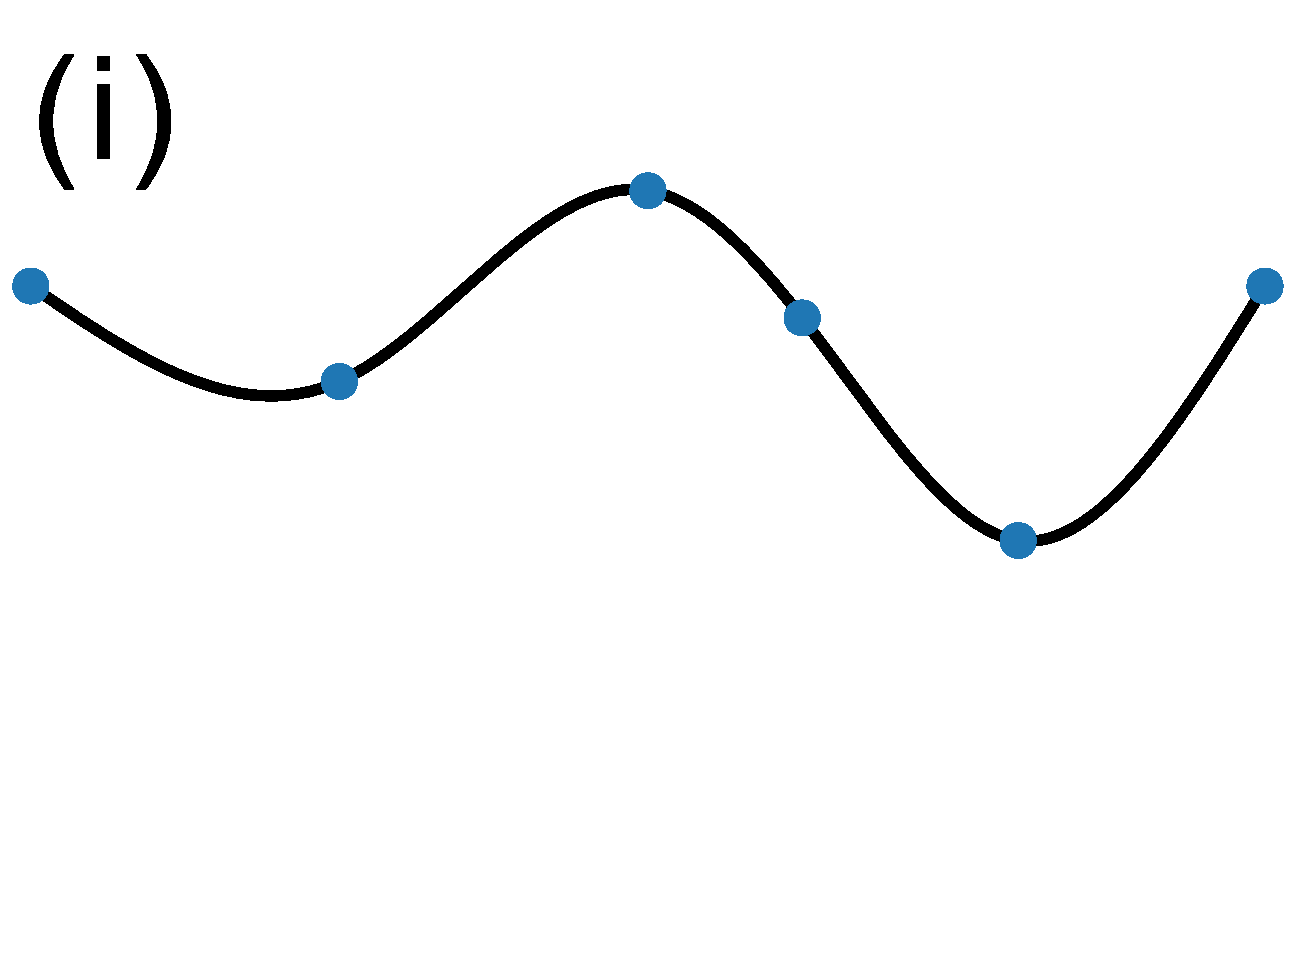
\includegraphics[scale=0.08]{content/images/spline_i.pdf}
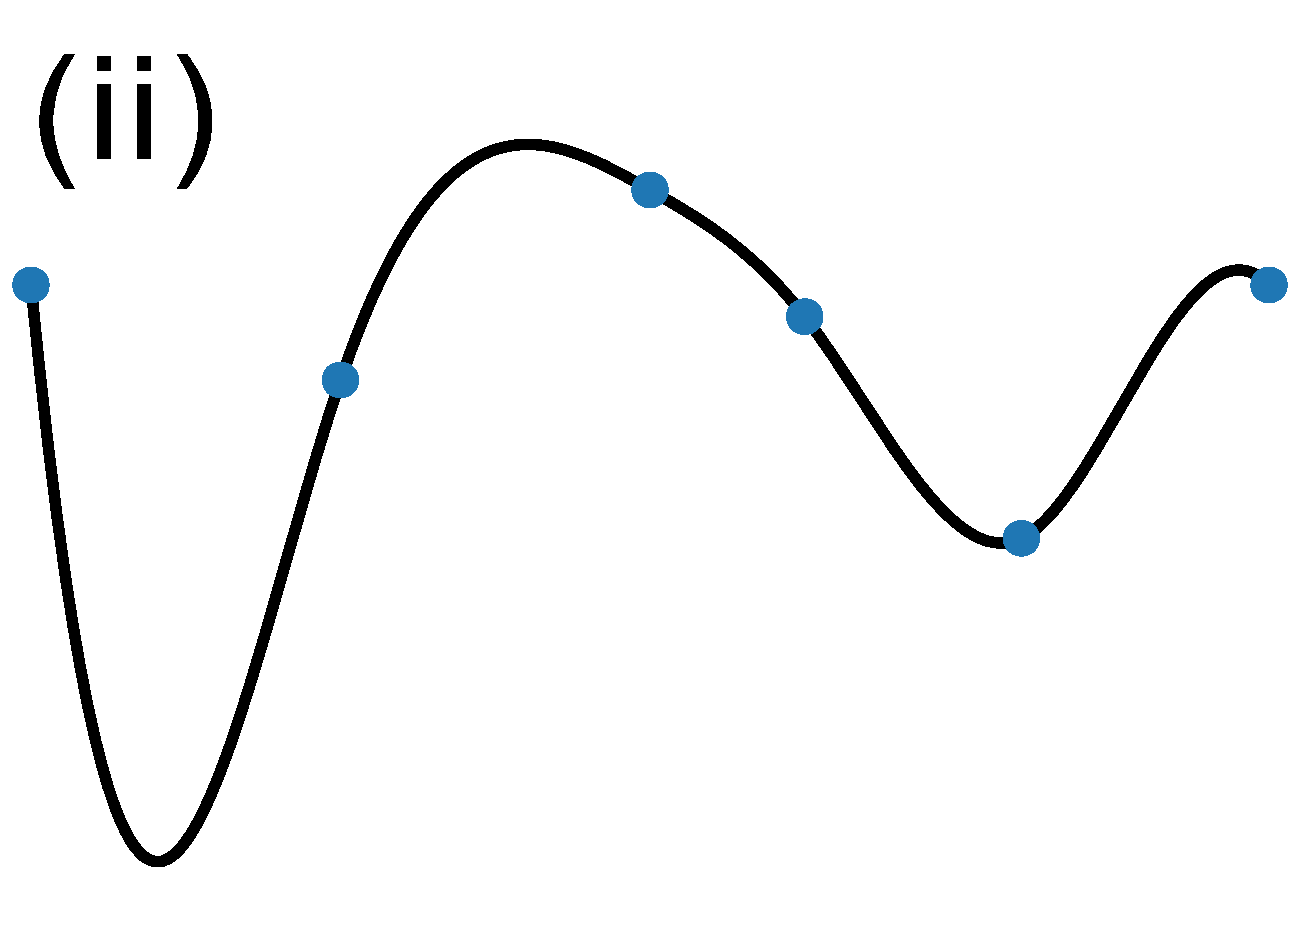
\includegraphics[scale=0.08]{content/images/spline_ii.pdf}
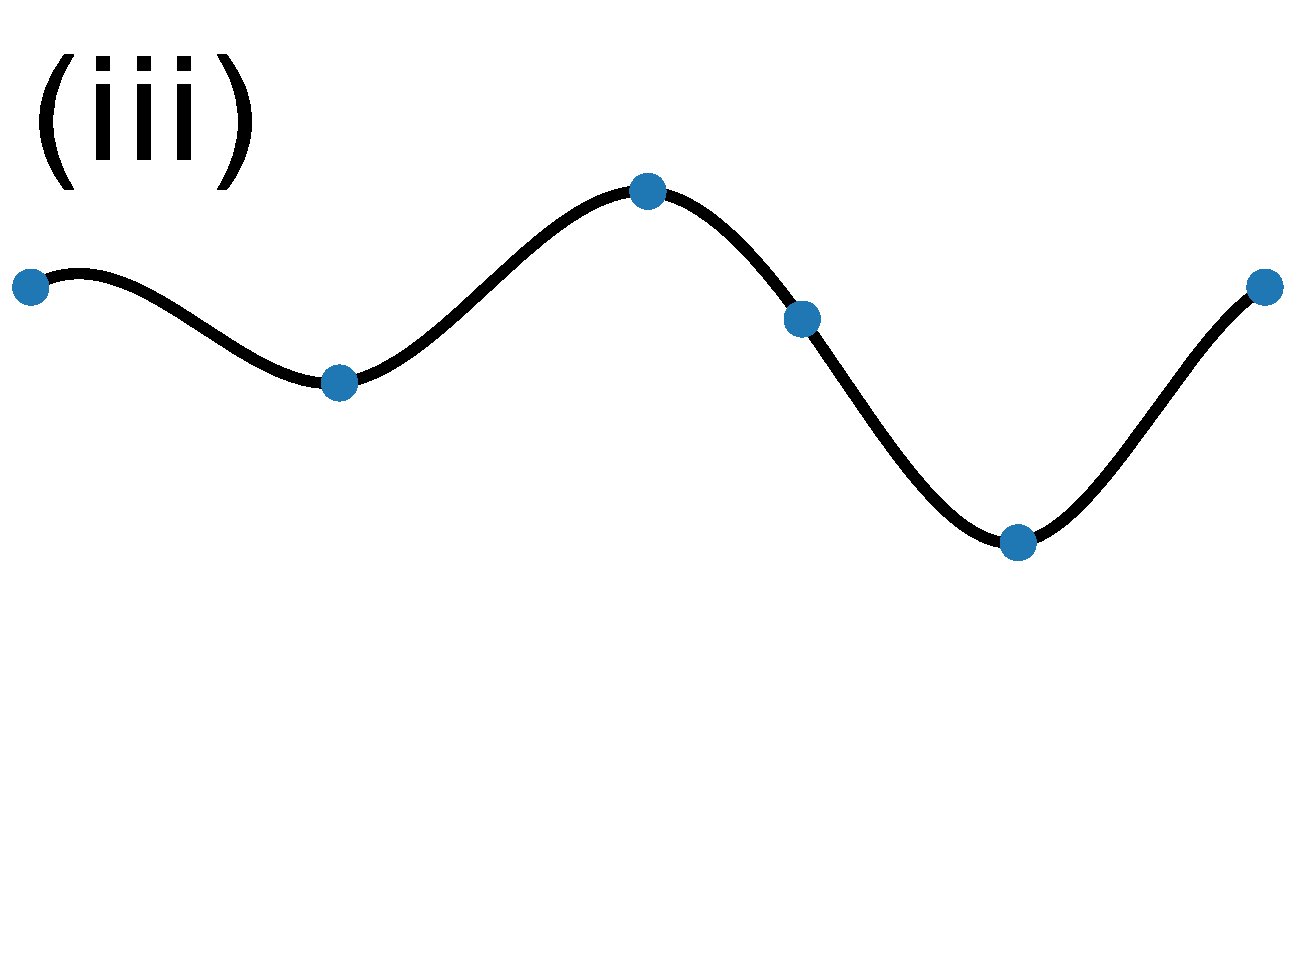
\includegraphics[scale=0.08]{content/images/spline_iii.pdf}\\
(i) natürlich, da Steigung an linken und rechtem RP $\approx$ konstant (ii) eingespannt, da nicht periodisch und nicht natürlich (iii) periodisch, da Steigung an Randpunkten $\approx$ identisch, RP: Randpunkt\\
%-----------------------------------------------------\\
-----------------------------------------------------\\
Knoten sym. $\leftrightarrow$ Ordnung p gerade. Es gilt $p \in (s, 2s]$. Da $2s$ eindeutig und Quadratur nicht identisch, gilt $p \in (s, 2s)$\\
-----------------------------------------------------\\
\textbf{Shiftmatrix}: $S = (e^N | e^1 | e^2 | ... | e^{N-1})$,\\ \hspace*{1mm}Iteration mit SV $y^0 = e^1$, konvergent?\\
\hspace*{1mm}\textbf{Lsg}: Iteration $y^{k+1} = Sy^k \rightarrow$ durchläuft \hspace*{1mm} $e^1 \rightarrow e^N \rightarrow ... \rightarrow e^1 \rightarrow$ nicht konvergent\\
-----------------------------------------------------\\
\pmb{$Q_wAQ_w$} $ = (I_k - 2ww^T)A(I_k - 2ww^T) \\= (A - 2ww^TA)(I_k -2ww^T) \\= A-2Aww^T - 2ww^TA + 4ww^TAww^T$\\
(V: $v = -2Aw$) $A + vw^T + wv^T - 2ww^Tvw^T$\\
(V: $\alpha -w^Tv$) $A + vw^T + wv^T + 2\alpha ww^T$\\
(V: $u = v + \alpha w)$ $A + uw^T + wu^T$\\
-----------------------------------------------------\\
\textbf{cg: Eigenwerte} Geg: A quad. sdp mit größtem EW $\lambda_1 > 1$ (alg. VF 1) und $|\lambda - 1| \leq \epsilon$. $\mathrm{Z\kern-.6em\raise-0.7ex\hbox{Z}}$: $||x^2 - x^*||_A \leq \epsilon||x^0 - x^*||_A$. \textbf{Lsg}: Sei $q_2(x) = \frac{1}{\lambda_1}(\lambda_1 - x)(1-x)$. Satz 39: $||x^2 - x^*|| \leq max|q_2(\lambda_j)|*||x^0 - x*||_A \\
\leq max |\frac{\lambda_1(1-\lambda_j)}{\lambda_1}|*||x^0 - x^*||_A \leq \epsilon||x^0 - x^*||_A$\\
$\mathrm{Z\kern-.6em\raise-0.7ex\hbox{Z}}$: k vers. EW $\Leftrightarrow$ exakte LSG nach k Schritten. \textbf{Lsg}: Sei $q_k(\lambda) = \prod_{j = 1}^k = \frac{\lambda_j - \lambda}{\lambda_j}$. Es gilt $q_k(0) = 1$ und $q_k(\lambda_j) = 0$. Satz 39: $||x^k - x^*||_A \leq max|q_k(\lambda_j)|*||x^0 - x^*||_A \\ = 0 \rightarrow x^k = x^*$ ist Lsg. des LGS\\
-----------------------------------------------------\\
Sei $Q_w = I_4 - 2ww^T$ die HHT mit 
$Q_wA $ \mbox{$= \{r_{11} , r_{12}^T \}, \{0_3 , A^{(1)}\}$ und A. Bestimme} \mbox{$r_{11}$. \textbf{Lsg}: $\text{Norm erster Spalte } = ||Q_wa^1||_2$} $ = ||r_{11}e^1||_2 = |r_{11}|$. Wähle VZ sodass im Zähler $a^1 - r_{11}e^1$ keine Auslöschung auftritt $\rightarrow$ Falls $a_{11}$ neg. wähle $r_{11}$ pos.\\
------ \textbf{Schritt im Newton-Verfahren} ------\\
$x \rightarrow \begin{pmatrix} x_1^2 x_2 - 1 \\ sin(x_2 \pi) \end{pmatrix}$ mit SW $x^0 = \begin{pmatrix} 0,5 \\ 2 \end{pmatrix}$. \textbf{Lsg}: $f'(x_1,x_2) = \begin{pmatrix} 2 \hspace*{3mm} 0.25\\0 \hspace*{3mm} \pi \end{pmatrix}$. Es gilt \mbox{$f'(x_1,x_2) \begin{pmatrix} d_1 \\ d_2 \end{pmatrix} = x^0$, $x = x^0 + d \rightarrow \begin{pmatrix} 0.75 \\ 2\end{pmatrix}$}\\
----------\textbf{Zusammenhang Normen}----------\
\mbox{$||x||_{\infty} = max_{1 \leq i \leq n}|x_i| = \sqrt{max_{1 \leq i \leq n}|x_i|^2}\leq$} \\
\mbox{$\sqrt{\sum_{i=1}^n|x_i|^2} = ||x||_2 \leq \sqrt{\sum_{i=1}^n} max_{1 \leq j \leq n |x_j|^2}$}\\
\mbox{$= \sqrt{n}*max_{1 \leq j \leq n}|x_j|^2 = \sqrt{n}||x||_{\infty}$}\\
-------- \textbf{Ableitungen und Sonstiges} --------\\
\mbox{$(a^x)' = (a^x) ln(a)$, \hspace{1.5mm}$\sqrt{x}' = \frac{1}{2\sqrt{x}}$, \hspace{1.5mm} GLHF :)}
\end{multicols*}
\end{document}